\documentclass[t]{beamer}

\subtitle{Diophantine Equations}

\usepackage{amsthm,amsmath,amsfonts,hyperref,graphicx,color,multicol,soul}
\usepackage{enumitem,tikz,tikz-cd,setspace,mathtools}

%%%%%%%%%%
%Beamer Template Customization
%%%%%%%%%%
\setbeamertemplate{navigation symbols}{}
\setbeamertemplate{theorems}[ams style]
\setbeamertemplate{blocks}[rounded]

\definecolor{Blu}{RGB}{43,62,133} % UWEC Blue
\setbeamercolor{structure}{fg=Blu} % Titles

%Unnumbered footnotes:
\newcommand{\blfootnote}[1]{%
	\begingroup
	\renewcommand\thefootnote{}\footnote{#1}%
	\addtocounter{footnote}{-1}%
	\endgroup
}

%%%%%%%%%%
%TikZ Stuff
%%%%%%%%%%
\usetikzlibrary{arrows}
\usetikzlibrary{shapes.geometric}
\tikzset{
	smaller/.style={
		draw,
		regular polygon,
		regular polygon sides=3,
		fill=white,
		node distance=2cm,
		minimum height=1in,
		line width = 2pt
	}
}
\tikzset{
	smsquare/.style={
		draw,
		regular polygon,
		regular polygon sides=4,
		fill=white,
		node distance=2cm,
		minimum height=1in,
		line width = 2pt
	}
}


%%%%%%%%%%
%Custom Commands
%%%%%%%%%%

\newcommand{\C}{\mathbb{C}}
\newcommand{\quats}{\mathbb{H}}
\newcommand{\N}{\mathbb{N}}
\newcommand{\Q}{\mathbb{Q}}
\newcommand{\R}{\mathbb{R}}
\newcommand{\Z}{\mathbb{Z}}

\newcommand{\ds}{\displaystyle}

\newcommand{\fn}{\insertframenumber}

\newcommand{\id}{\operatorname{id}}
\newcommand{\im}{\operatorname{im}}
\newcommand{\lcm}{\operatorname{lcm}}
\newcommand{\Aut}{\operatorname{Aut}}
\newcommand{\Inn}{\operatorname{Inn}}

\newcommand{\blank}[1]{\underline{\hspace*{#1}}}

\newcommand{\abar}{\overline{a}}
\newcommand{\bbar}{\overline{b}}
\newcommand{\cbar}{\overline{c}}

\newcommand{\nml}{\unlhd}

%%%%%%%%%%
%Custom Theorem Environments
%%%%%%%%%%
\theoremstyle{definition}
\newtheorem{exercise}{Exercise}
\newtheorem{question}[exercise]{Question}
\newtheorem{warmup}{Warm-Up}
\newtheorem*{exa}{Example}
\newtheorem*{disc}{Group Discussion}
\newtheorem*{recall}{Recall}
\renewcommand{\emph}[1]{{\color{blue}\texttt{#1}}}

\definecolor{Gold}{RGB}{237, 172, 26}
%Statement block
\newenvironment{statementblock}[1]{%
	\setbeamercolor{block body}{bg=Gold!20}
	\setbeamercolor{block title}{bg=Gold}
	\begin{block}{\textbf{#1.}}}{\end{block}}
\newenvironment{goldblock}{%
	\setbeamercolor{block body}{bg=Gold!20}
	\setbeamercolor{block title}{bg=Gold}
	\setbeamertemplate{blocks}[shadow=true]
	\begin{block}{}}{\end{block}}
\newenvironment{defn}{%
	\setbeamercolor{block body}{bg=gray!20}
	\setbeamercolor{block title}{bg=violet, fg=white}
	\setbeamertemplate{blocks}[shadow=true]
	\begin{block}{\textbf{Definition.}}}{\end{block}}
\newenvironment{nb}{%
	\setbeamercolor{block body}{bg=gray!20}
	\setbeamercolor{block title}{bg=teal, fg=white}
	\setbeamertemplate{blocks}[shadow=true]
	\begin{block}{\textbf{Note.}}}{\end{block}}
\newenvironment{blockexample}{%
	\setbeamercolor{block body}{bg=gray!20}
	\setbeamercolor{block title}{bg=Blu, fg=white}
	\setbeamertemplate{blocks}[shadow=true]
	\begin{block}{\textbf{Example.}}}{\end{block}}
\newenvironment{blocknonexample}{%
	\setbeamercolor{block body}{bg=gray!20}
	\setbeamercolor{block title}{bg=purple, fg=white}
	\setbeamertemplate{blocks}[shadow=true]
	\begin{block}{\textbf{Non-Example.}}}{\end{block}}
\newenvironment{thm}[1]{%
	\setbeamercolor{block body}{bg=Gold!20}
	\setbeamercolor{block title}{bg=Gold}
	\begin{block}{\textbf{Theorem #1.}}}{\end{block}}


%%%%%%%%%%
%Custom Environment Wrappers
%%%%%%%%%%
\newcommand{\exer}[1]{
	\begin{exercise}
		#1
	\end{exercise}
}
\newcommand{\exam}[1]{
\begin{blockexample}
	#1
\end{blockexample}
}
\newcommand{\nexam}[1]{
\begin{blocknonexample}
	#1
\end{blocknonexample}
}
\newcommand{\enumarabic}[1]{
	\begin{enumerate}[label=\textbf{\arabic*.}]
		#1
	\end{enumerate}
}
\newcommand{\enumalph}[1]{
	\begin{enumerate}[label=(\alph*)]
		#1
	\end{enumerate}
}
\newcommand{\bulletize}[1]{
	\begin{itemize}[label=$\bullet$]
		#1
	\end{itemize}
}
\newcommand{\circtize}[1]{
	\begin{itemize}[label=$\circ$]
		#1
	\end{itemize}
}
\newcommand{\slide}[1]{
	\begin{frame}{\fn}
		#1
	\end{frame}
}
\newcommand{\slidec}[1]{
\begin{frame}[c]{\fn}
	#1
\end{frame}
}
\newcommand{\slidet}[2]{
	\begin{frame}{\fn\ - #1}
		#2
	\end{frame}
}


\newcommand{\startdoc}{
		\title{Math 341: Classical Number Theory}
		\author{Mckenzie West}
		\date{Last Updated: \today}
		\begin{frame}
			\maketitle
		\end{frame}
}

\newcommand{\topics}[2]{
	\begin{frame}[c]{\insertframenumber}
		\begin{block}{\textbf{Last Section.}}
			\begin{itemize}[label=--]
				#1
			\end{itemize}
		\end{block}
		\begin{block}{\textbf{This Section.}}
			\begin{itemize}[label=--]
				#2
			\end{itemize}
		\end{block}
	\end{frame}
}
\usepackage{pgfplots}

\begin{document} 
	\startdoc
	
	\topics{
		% Last Time
		\item More with gcds
		\item If $a^n|b^n$ then $a|b$
	}
	{
		% This time
		\item Diophantine Equations of the form $ax+by=c$
		\item Solving Diophantine Equations
	}

\slide{
	\begin{defn}
		The \emph{Euclidean algorithm} is a method from computing $\gcd(a,b)$. Assume for simplicity that $a\geq b>0$ since $\gcd(|a|,|b|)=\gcd(a,b)$ and $\gcd(a,0)=a$ if $a>0$. By the division algorithm, we can write
		
			\[
			\begin{array}{rcll}
			a&=&q_0b+r_1 & 0<r_1<b\\
			b&=&q_1r_1+r_2 & 0<r_2<r_1\\
			r_1&=&q_2r_2+r_3 & 0<r_3<r_2\\
			r_2&=&q_3r_3+r_4 & 0<r_4<r_3\\
			&\vdots\\
			r_{n-2}&=&q_{n-1}r_{n-1}+r_n & 0<r_n<r_{n-1}\\
			r_{n-1}&q_nr_n+0.
			\end{array}
			\]
		Then \fbox{$r_n=\gcd(a,b)$}.
	\end{defn}
}
\slide{
	\begin{statementblock}{Theorem 2.9}
		The linear Diophantine equation  $ax+by=c$ has a solution if and only if $d|c$, where $d=\gcd(a,b)$. If $x_0,y_0$ is any particular solution of this equation ,then all other solutions are given by
			\[x=x_0+\left(\frac{b}{d}\right)t,\quad y=y_0-\left(\frac{a}{d}\right)t,\]
		where $t$ is an arbitrary integer.
	\end{statementblock}
	\begin{defn}
		To \emph{solve} a Diophantine equation is to find all possible integer$^*$ values that satisfy the equation.
	\end{defn}
}
\slide{
	\begin{exercise}
		Which of the following Diophantine equations can be solved?
		\enumalph{
			\item $900x+6y=36$
			\item $300x+225y=4$
			\item $100x+90y=30$
			\item $36x+18y=50$
	}
	\end{exercise}
}
\slide{
	\begin{exercise}
		Solve the Diophantine equation
		\[100x+90y=30.\]
	\end{exercise}
}
\slide{
	\begin{exercise}
		Solve the Diophantine equation
		\[12012x+3575y=1859.\]
		
		\fbox{
		$\begin{array}{rcll}
		12012&=&3\cdot 3575+1287\\
		3575&=&2\cdot 1287+1001\\
		1287&=&1\cdot 1001 + 286\\
		1001&=&3\cdot 286+143\\
		286&=&2\cdot 143
		\end{array}
		$
		}
	\end{exercise}
}
\slide{
\begin{exercise}
	Solve this problem posed by B\'ezout in 1766.
	
	You have a bag of silver coins, each coin weighing 17 ounces of silver. A merchant has a bag of silver coins, each weighing 11 ounces. You wish to pay the merchant 542 ounces of silver.  How many 17-ounce coins should you give the merchant, and how many 11-ounce coins should the merchant give you?
	
	What is the smallest number of coins that can be exchanged in this transaction?
\end{exercise}
}
\slide{
	\begin{exercise}
		A farmer purchased 100 head of livestock for a total cost of \$4000. Prices were as follows: calves, \$120 each; lambs \$50 each; piglets \$25 each. If the farmer obtained at least one animal of each type, how many of each did they buy? 
	\end{exercise}
}
\slide{
	\begin{exercise}
		Solve this problem posed by Euler in 1770.
		
		Divide 100 into two summands such that one is divisible by 7 and the other by 11.
	\end{exercise}
}
\slide{
	Diophantine equations as geometric objects.
	
	Assume $a,b,c>0$, then $ax+by=c$ is equivalent to
		$$y=-\frac{a}{b}x+\frac{c}{b},$$
	which is a line that has $y$-intercept $\frac{c}{b}$ and slope $-\frac{a}{b}$.
	
\begin{center}
	\resizebox{0.5\textwidth}{!}{
		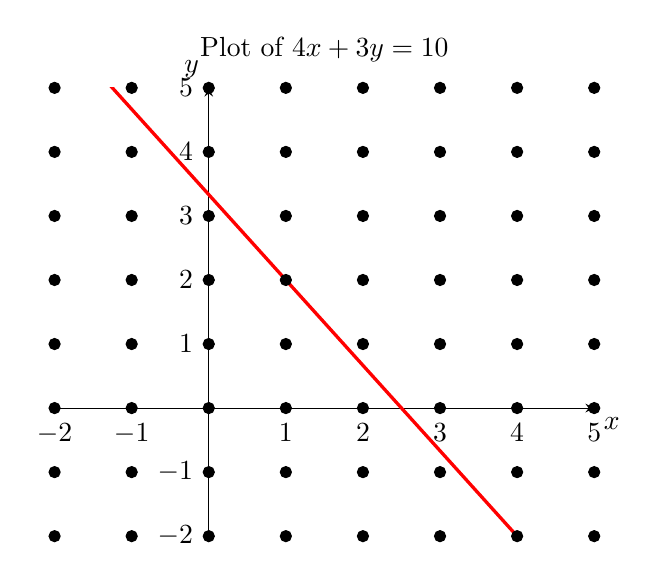
\begin{tikzpicture}
	\begin{axis}[
	title={Plot of $4x+3y=10$},
	axis x line=center,
	axis y line=center,
	xmin=-2, xmax=5,
	ymin=-2, ymax=5,  
	xtick={-2,-1,...,5},
	ytick={-2,-1,...,5},
	xlabel={$x$},
	ylabel={$y$},
	xlabel style={below right},
	ylabel style={above left},
	ymajorgrids=false,
	xmajorgrids=false,
	grid style=dashed,
	]
	\addplot [
	domain=-10:10, 
	samples=100, 
	color=red,
	very thick
	]
	{-4/3*x+10/3};
	% points (1,2) and (2.5,0) => slope -4/3
	\foreach \i in {-2,...,5}{
		\foreach \j in {-2,...,5}{
			\addplot[only marks,mark=*,] coordinates {
				(\i,\j)};
	}}
	\end{axis}
	\end{tikzpicture}
}
\end{center}
}
\slide{
We can also consider other lattices, such as the half-integer lattice.

\begin{center}
	\resizebox{0.5\textwidth}{!}{
		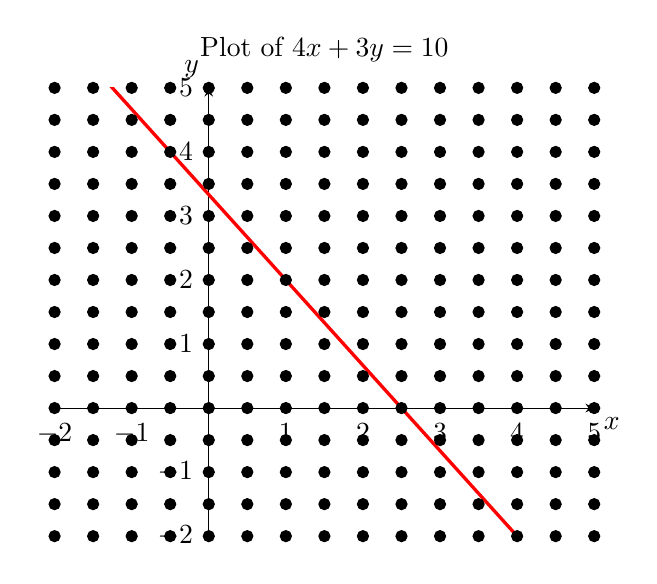
\begin{tikzpicture}
		\begin{axis}[
		title={Plot of $4x+3y=10$},
		axis x line=center,
		axis y line=center,
		xmin=-2, xmax=5,
		ymin=-2, ymax=5,  
		xtick={-2,-1,...,5},
		ytick={-2,-1,...,5},
		xlabel={$x$},
		ylabel={$y$},
		xlabel style={below right},
		ylabel style={above left},
		ymajorgrids=false,
		xmajorgrids=false,
		grid style=dashed,
		]
		\addplot [
		domain=-10:10, 
		samples=100, 
		color=red,
		very thick
		]
		{-4/3*x+10/3};
		% points (1,2) and (2.5,0) => slope -4/3
		\foreach \i in {-4,...,10}{
			\foreach \j in {-4,...,10}{
				\addplot[only marks,mark=*,] coordinates {
					(\i/2,\j/2)};
		}}
		\end{axis}
		\end{tikzpicture}
	}
\end{center}
}

\end{document}

